\chapter{Intrusion Detection Systems}
\minitoc
In \label{chap:IDS} this chapter we will define Intrusion Detection Systems, present an overview of the different types of Intrusion Detection Systems
%Host based and network based IDS
%network based IDS: signature based and anomaly based IDS

\section{The problem}

Some more itro needed\ldots.

Let us first provide an analogue, real world example of the security problem. Suppose that one has just bought a brand new luxury sedan. After parking it into the garage box, one might decide to install new security locks on the garage box's door, because the old ones do not use the up-to-date security mechanisms. After making a call to the locksmith who installs the new locks, you are the only one possessing the new keys.

After all that said and done, one decides to go on vacation. When returning home after a few weeks because of nostalgia, one decides to make a ride is his new car. However, when opening the door of the garage box, one does not see his brand new car as expected, but rather an empty garage box. What's worse is that one does not only see an empty box, but also some shards of glass on the floor. That led one to believe that someone broke into your garage box, stole your car and vandalized some of your possessions.

A few weeks before, one received a brochure of a company that installs burglar alarms. However, one threw it away. The installation and monitoring would have cost just 20 dollars a month. Neglecting to install the system is a secret one would have to leave with for the rest of one's life.

Could one have prevented the burglary from happening if one had installed the alarm?  Maybe not completely, but no doubt the damage would be less. \\ \\
This real life example is the same analogy of what might happen to one's computer network. What's more is that the thief may be at one's network for a long time without noticing him. Firewalls are doing (if properly configured) a good job guarding one's front door, but do not alert in case there is a back door or hole in one's infrastructure. So it is important to realize that a firewall is not an intrusion detection system.

\section{Intrusion Detection}

The \label{sec:ID} above example illustrates the need for intrusion detection systems. An IDS is the technology aimed at providing a precise detection measure on any intrusion attempt. We distinguish two different types of IDS: host based (HIDS) and network based NIDS).

A host intrusion detection system takes a snapshot of your existing system files and matches it to the previous snapshot. If the critical system files were modified or deleted, the alert is sent to the administrator to investigate. The example of the HIDS can be seen on the mission critical machines, that are not expected to change their configuration.

A HIDS is  is a sort of indoor surveillance system thats examines the system integrity for any signs of intrusions. an HIDS usually is software installed within a monitored system and placed on business-critical systems. Some of the system variables that HIDSs are likely to monitor are

A NIDS is a sort of outdoor surveillance system that examines the data traffic passing troughout a network for any signs of intrusion. The IDS consists of two parts: the console and the sensor. The console is a management station that manages the incoming alerts and updates signatures on the sensor. The sensor is a monitoring agent (station) that is put onto any monitored network and raises alarms to the management station if any data traffic matches its signature database. Advantages of NIDS are the easy deployment (it doesn't affect any existing system), detection of network-based attacks such as SYN floods, fragmented packets, etc\ldots and earlier detection of reconnaissance type of attack. Disadvantages however include more proneness to false alarms compared to a HIDS, because of it's impossibility to indicate whether or not the attack was successful. Further correlation to multiple sources of information is still required to determine if an attack attempt was successful or not and to determine how far a particular attack has reached.

\subsection{What is not an IDS?}

Following devices, tools and software are not IDSs \citep{windowssecurity}:
\begin{enumerate}
\item Vulnerability assessment tools that check for bugs in operating systems and network services.
\item Anti-virus software to detect viruses, trojan horses, worms, etc\ldots.
\item Firewalls
\item Cryptographic systems such as VPN, SSL and RADIUS.
\end{enumerate}

\section{Architecture of intrusion detection systems}

An intrusion detection system always has its core element: the sensor. It is responsible for detecting intrusions and contains descision-making mechanisms. The sensor receives data from three information sources: its own IDS knowledge database, audit trails and syslog. This information creates the basis for a further descision-making process \citep{windowssecurity}.

\begin{figure}[h]
    \centering
    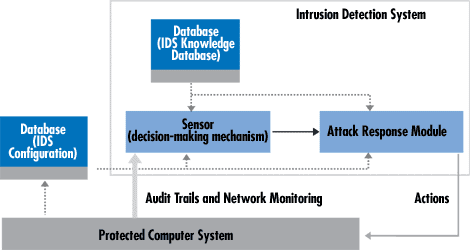
\includegraphics[width=0.85\textwidth]{IDS_1.jpg}
    \caption{Example of a Network-based Intrusion Detection System}
    \label{fig:NIDS}
\end{figure}

The sensor is integrated with the component responsible for data collection (Fig.4) — an event generator. The collection manner is determined by the event generator policy that defines the filtering mode of event notification information. The event generator (operating system, network, application) produces a policy-consistent set of events that may be a log (or audit) of system events, or network packets. This, set along with the policy information can be stored either in the protected system or outside. In certain cases, no data storage is employed for example, when event data streams are transferred directly to the analyzer. This concerns the network packets in particular \citep{windowssecurity1}.

\begin{figure}[h]
    \centering
    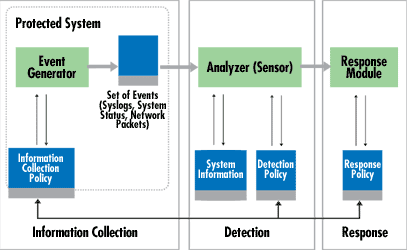
\includegraphics[width=0.85\textwidth]{IDS_2.jpg}
    \caption{Example of a Network-based Intrusion Detection System}
    \label{fig:NIDS}
\end{figure}

The role of the sensor is to filter information and discard any irrelevant data obtained from the event set associated with the protected system, thereby detecting suspicious activities. The analyzer uses the detection policy database for this purpose. The latter comprises the following elements: attack signatures, normal behavior profiles, necessary parameters (for example, thresholds). In addition, the database holds IDS configuration parameters, including modes of communication with the response module. The sensor also has its own database containing the dynamic history of potential complex intrusions (composed from multiple actions) \citep{windowssecurity1}.

\section{The different types of IDS}

\subsection{Classification based on detection method}

There exist two main types of intrusion detection systems: signature-based (SBS) and anomaly-based (ABS). Signature-based intrusion detection systems rely on pattern-matching techniques: they contain a database of signatures of known attacks and try to match these data against the analyzed data. When a match is found, an alarm is raised \citep{Roberto}.

On the other hand, anomaly-based intrusion detection systems first build
a statistical model describing the normal network traffic, then reports any behaviour that significantly deviates from the model as an attack \citep{Roberto}. They explore issues in intrusion detection associated with deviations from normal system or user behavior \citep{windowssecurity2}.

Simply stated, anomaly based systems have the advantage that they can detect zero-day attacks \footnote{Zero-day attack: the term zero-dat attack is derived from the age of the exploit. A zero day exploit is when the exploit for the vulnerability is created before, or on the same day as the vulnerability is learned about by the vendor. By creating a virus or worm that takes advantage of a vulnerability the vendor is not yet aware of and for which there is not currently a patch available, the attacker can wreak maximum havoc \citep{Zero}.}, since novel attacks can be detected as soon as they take place \citep{Roberto}.

On the other hand, anomaly-based intrusion detection systems require a training phase and a careful setting of the detection threshold, which makes their deployment more complex \citep{Roberto}.

\subsubsection{Anomaly-Based Intrusion Detection Systems}

We will provide a brief description about ABSs.There exist different types of ABSs, but in general terms, they all consist of the following basic parts:
\begin{description}
\item[Training / learning phase] The normal behaviour of the system is characterized and a corresponding model is built. This can be done automatically or manually, depending on the type of ABS used.
\item[Detection phase] Once the model is built, it is compared with the observed traffic. If the difference found exceeds a pre-defined threshold value, an alarm will be triggered.
\item[Threshold value]
\end{description}

As previously mentioned, there exist three types of ABSs; they can be classified according to
\begin{itemize}
\item The underlying algorithm they use.
\item Whether they analyse the payload of each package singularly or of the whole connection.
\item The kind of data they analyse. More precise: whether they focus on the packet header or on the payload.
\end{itemize}
There exist various possible approaches of underlying algorithms, with algorithms based on statistical models and those based on neural networks\footnote{Neural network:} being the most popular. 

According to \citep{Debar} more than 50\% of existing ABSs is statistic-based. Therefore making the algorithms based on statistical models the most widely used. In these systems, the algorithm first builds a statistical model (the training phase) of the clean, attack-free network and later, in the detection phase , the incoming data is compared to the model. When the incoming data differs too much compared to that model, the incoming data is considered anomalous. I.e., it is considered as an attack \footnote{The statistical model uses a so-called distance function. When the distance measured of the incoming data exceeds a pre-defined threshold value, an alarm is raised.} \citep{Roberto}.

ABSs based on neural networks work in a similar way as they also have a learning phase, a detection phase and a threshold value, but instead of building a statistical model, they train a neural network which is in charge of distinguishing regular traffic from anomalous one \citep{Roberto}. 

In comparision to signatured based intrusion detection systems, the main benefit of anomaly-based detection techniques is their potential to detect previously unseen
intrusion events. However, and despite the likely inaccuracy in formal signature specifications, the rate of false positives in anomaly-based systems is usually higher than in signature-based ones \citep{CandS}.

As my paper focuses on the signature-based intrusion detection systems, we won't look further into the subject of anomaly-based IDSs.

\subsubsection{Signature-Based Intrusion Detection Systems}

Signature-based schemes seek defined patterns, or signatures, within the analyzed data. For this purpose, a signature database corresponding to known attacks is specified a priori \citep{CandS}.

The signature based intrusion detection system analyzes information it gathers and compares it to a large database of attack signatures. The system looks for a specific attack that has already been documented \citep{Patent}.

Compare to an anti-virus: virusdefinities bijwerken, \ldots.

Signature-based schemes provide very good detection results for specified, well-known attacks. However, they are not capable of detecting new, unfamiliar intrusions, even if they are built as minimum variants of already known attacks \citep{CandS}.

network-based signature matching in which the system inspects network traffic for matches against exact, precisely-described patterns. While NIDSs use different abstractions for defining such patterns, most of the time the term signature refers to raw byte sequences. Typically, a site deploys a NIDS where it can see network traffic between the trusted hosts it protects and the untrusted exterior world, and the signature-matching NIDS inspects the passing packets for these sequences. It generates an alert as soon as it encounters one. Most commercial NIDSs follow this approach [19], and also the most well-known freeware NIDS, Snort [29]. As an example,to detect the buffer overflow described in [9], Snort’s signature \#1808 looks for the byte pattern 0xC0505289E150515250B83B000000CD80
[2] in Web requests. Keeping in mind that there are more general forms of signatures used in intrusion detection as well some of which we briefly discuss in 2 in this paper we adopt this common use of the term signature.

Signature-matching in this sense has several appealing properties. First, the underlying conceptual notion is simple: it is easy to explain what the matcher is looking for and why, and what sort of total coverage it provides. Second, because of this simplicity, signatures can be easy to share, and to accumulate into large “attack libraries.” Third, for some signatures, the matching can be quite tight: a match indicates with high confidence that an attack occurred.
On the other hand, signature-matching also has significant limitations. In general, especially when using tight signatures, the matcher has no capability to detect attacks other than those for which it has explicit signatures; the matcher will in general completely miss novel attacks, which, unfortunately, continue to be developed at a brisk pace. In addition, often signatures are not in fact “tight.” For example, the Snort signature \#1042 to detect an exploit of CVE-2000-0778 [9] searches for “Translate: F” in Web
requests; but it turns out that this header is regularly used by certain applications. Loose signatures immediately raise the major problem of false positives: alerts that in fact do not reflect an actual attack. A second form of false positive, which signature matchers likewise
often fail to address, is that of failed attacks. Since at many sites attacks occur at nearly-continuous rates, failed attacks are often of little interest. At a minimum, it is important to distinguish between them and successful attacks.

\subsection{Classification based on protective system}

\subsubsection{HIDS}

As described in section \ref{sec:ID}, a host-based intrusion detection system or HIDS monitors activity on a single host. They are aimed at collecting information about activity on a particular single system, or host \citep{Host1} and is therefore installed on a single system, which is in most cases a business-critial system or server. Whereas a HIDS resides on a single computer, a network-based intrusion detection system or NIDS is installed on, for example, routers \citep{windowssecurity2}.

The term `host' or `single system', refers to an individual computer, thus a seperate agent (the actual HIDS program) would be needed for every machine. Agents work by collecting data about events taking place on the system being monitored. This data is recorded by operating system mechanisms called audit trails or event logs\citep{Host1, Host2}.  Other sources from which a host-based agent can obtain data, include system logs, other logs generated by operating system processes, and contents of objects not reflected in standard operating system audit and logging mechanisms \citep{Host1}.

However, there are some issues related to audit trail (event log) processing. First, storing audit trail reports in a single file must be avoided since intruders may use this feature to make unwanted changes. It is far better to keep a certain number of event log copies spread over the network, though it would imply adding some overheads to both the system and network \citep{windowssecurity2}.

Second, recording every event possible means a noticeable consumption of system resources. Specifying which events are to be audited is difficult because certain types of attacks may pass undetected. It is also difficult to predict how large audit files can be - through experience one can only make a rough estimate \citep{windowssecurity2}.
Therefore, audit trails can be very costy, taking up significant storage space as well as increasing hosting machine load \citep{Host1}.

Host-based intrusion detection systems can be divided into four types \citep{Report}:
\begin{description}
\item[File system monitoring] \hfill \\
File system monitoring is a system that checks the integrity of files and directories. HIDS implementations that use filesystem monitoring compare files on a regulary basis with previously gathered information about these files, such as size, owner and last modification date. This way, when an attacker gains access to those files and changes them, it will be detected. File system monitoring can check files for different characteristics inlucding, but not limited to: permissions, inode number, Owner/Group, size, etc\ldots.
\item[Logfile analysers] \hfill \\
Logfile analysers analyse logfiles for patterns indicating suspicious activity (= intrusions). By analyzing logfiles and determing if intrusion attempts were logged, an IDS can warn system administrators.
\item[Connection analysers] \hfill \\
A connection analyser monitors connection attempts to and from a host. They detect incoming network connections to the host they run on. Network-based intrusion detection systems (NIDS) as discussed in section \ref{subsub:NIDS} such as Snort use this approach \citep{Snort}.
\item[Kernel-based IDSs] \hfill \\
Kernel-based IDSs detect malicious activity on a kernel level. It is an adoption to or adoption of an existing kernel to have the kernel itself detect intrusions. Anomaly detection is a popular detection method used in Kernel-based IDSs. There exist various anomaly detection methods: anomaly detection based on a user's system usage, anomaly detection on the order of system calls in processes and anomaly detection on the arguments of system calls in processes.
\end{description}

\begin{figure}[h]
    \centering
    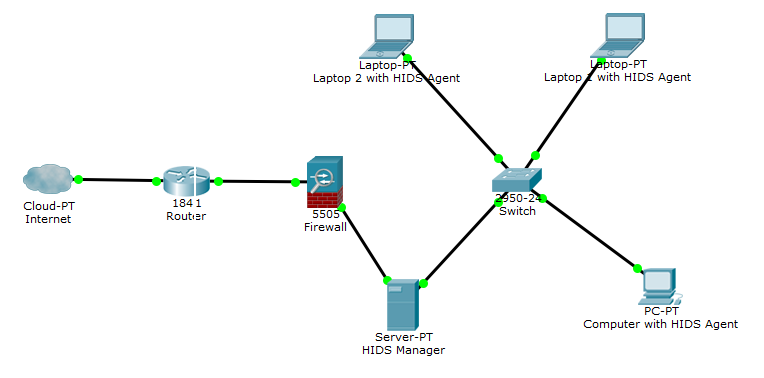
\includegraphics[width=0.85\textwidth]{HIDS.jpg}
    \caption{Example of a Host-based Intrusion Detection System}
    \label{fig:HIDS}
\end{figure}

Since Host-based IDSs are not designed to `see' network traffic, they are unable detect and report intrusions on a local network. That's when NIDS or Network-based intrusion detection systems come to help.

\subsubsection{NIDS}

A NIDS \label{subsub:NIDS} produces data about the local network. In particular, about local network usage. They collect information from the network itself, rather than from each seperate host \citep{Host2}. The NIDS analyze all network packets that reach the monitored network interface running in promiscuous mode \footnote{Promiscuous mode allows a network device to intercept and read each packet that arrives in its entity. I.e., it causes the network card to pass all traffic it receives to the CPU rather than passing only the frames that the controller is intended to receive. In a LAN, promiscuous mode is a mode of operation in which every data packet transmitted on the network can be received and read by the network adapter. Needless to say, promiscuous mode is used to monitor network traffic - and activity \citep{Prom}.}. Previous statement defines that a NIDS can not only be installed on a router, but also on a server that has a network interface card (NIC) operating in promiscuous mode.

Once a packet reaches the NIC, its header and content information is inspected \citep{Host2}. Signature-based IDSs come equipped with attack signatures, which are rules on what will constitute an attack. The sensors then compare these signatures to the traffic  that they capture. This method is known as packet sniffing \citep{Sniffing}.

\begin{figure}[h]
    \centering
    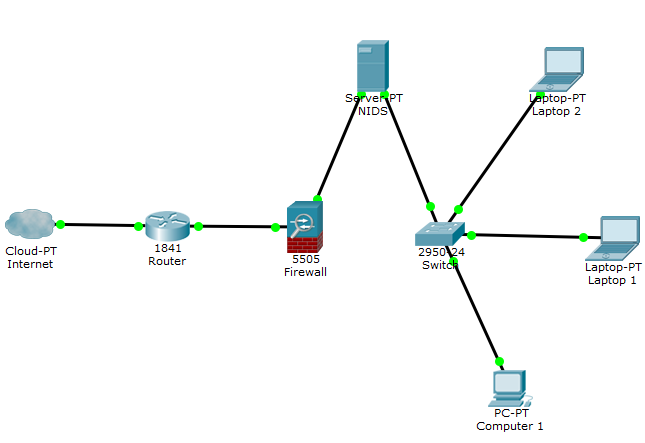
\includegraphics[width=0.85\textwidth]{NIDS.jpg}
    \caption{Example of a Network-based Intrusion Detection System}
    \label{fig:NIDS}
\end{figure}

\subsection{Classification based on structure}

\subsubsection{Centralised}

\subsubsection{Distributed}

A Distruibuted intrusion detection system or dIDS can be defined as ``multiple intrusion detection Systems spread over a large network, 
all of which communicate with each other, or with a central server that facilitates advanced network monitoring, incident analysis and instant attack data'' \citep{DIDS}.

